\documentclass[aspectratio=169,10pt]{beamer}
\usetheme{Madrid}
\usecolortheme{seahorse}
\useinnertheme{circles}
\useoutertheme{infolines}

\usepackage[utf8]{inputenc}
\usepackage{amsmath,amssymb}
\usepackage{booktabs}
\usepackage{graphicx}
\usepackage{xcolor}

\graphicspath{{../output/figures/}}

\setbeamertemplate{navigation symbols}{}
\setbeamercovered{transparent}
\setbeamerfont{footline}{size=\fontsize{6}{8}\selectfont}

\definecolor{accent}{RGB}{52,113,168}
\definecolor{warm}{RGB}{168,52,52}
\definecolor{green}{RGB}{58,138,58}
\setbeamercolor{title}{fg=accent}
\setbeamercolor{frametitle}{fg=accent}
\setbeamercolor{structure}{fg=accent}

\title[SNA Project 13]{Twitter COVID-19 Network Analysis}
\subtitle{Hashtag Co-occurrence, Temporal Decomposition\\
and Negative-Sentiment Propagation}
\author[M. Mandz\'{a}k]{Mat\'{u}\v{s} Mandz\'{a}k\\
\texttt{matus.mandzak@student.oulu.fi}}
\institute[Oulu]{Group 13 \textendash{} Faculty of ITEE, University of Oulu}
\date{Social Network Analysis \textendash{} Project 13}

\begin{document}

% ---------------------------------------------------------------- 1. Title
\begin{frame}
  \titlepage
  \begin{center}
    \footnotesize\href{https://github.com/MatusMandzak/sna-project}%
      {github.com/MatusMandzak/sna-project}
  \end{center}
\end{frame}

% ---------------------------------------------------------------- 2. Problem
\begin{frame}{Problem statement}
  \begin{block}{Project 13}
    Build a hashtag-co-occurrence graph from
    \textbf{TweetsCOV19} (Oct--Nov~2019), characterise it
    statically and over time, and test whether negative
    sentiment propagates like an SIS contagion.
  \end{block}
  \vfill
  \begin{columns}[T,onlytextwidth]
    \column{0.5\linewidth}
    \textbf{Static}
    \begin{itemize}\itemsep2pt
      \item \(|V|, |E|\), components, degree centrality
      \item top-3 connected components
      \item degree-centrality CDF
      \item power-law fit + \(R^{2}\)
    \end{itemize}
    \column{0.5\linewidth}
    \textbf{Temporal}
    \begin{itemize}\itemsep2pt
      \item 10 equal time increments
      \item per-increment subgraph metrics
      \item triangle evolution
      \item sentiment evolution
      \item SIS contagion calibration
    \end{itemize}
  \end{columns}
\end{frame}

% ---------------------------------------------------------------- 3. Dataset
\begin{frame}{Dataset}
  \begin{columns}[T,onlytextwidth]
    \column{0.55\linewidth}
    \begin{itemize}\itemsep4pt
      \item \textbf{TweetsCOV19} part 1\\(Oct 2019 -- Apr 2020)
      \item gzip TSV, 820~MB compressed,
            \(\sim\)8.15~M lines
      \item streaming filter on the timestamp column
      \item kept \textbf{287\,990} tweets in Oct--Nov 2019
            from \textbf{188\,649} users
      \item \textbf{764\,341} hashtag instances over
            \textbf{209\,330} unique tags
    \end{itemize}
    \vspace{4pt}
    \alert{Pre-pandemic window} -- \texttt{\#covid19} not yet
    in the popular tail.
    \column{0.45\linewidth}
    \scriptsize
    \begin{tabular}{lr}
      \toprule
      Hashtag & Tweets \\
      \midrule
      \texttt{\#china} & 7\,134 \\
      \texttt{\#healthcare} & 4\,835 \\
      \texttt{\#hongkong} & 4\,050 \\
      \texttt{\#hongkongprotests} & 2\,785 \\
      \texttt{\#strongertogether} & 2\,623 \\
      \texttt{\#standwithhongkong} & 2\,563 \\
      \texttt{\#epsteincoverup} & 2\,079 \\
      \texttt{\#chinazi} & 1\,879 \\
      \texttt{\#mamavote} & 1\,833 \\
      \bottomrule
    \end{tabular}
  \end{columns}
\end{frame}

% ---------------------------------------------------------------- 4. Pipeline
\begin{frame}{Pipeline}
  \footnotesize
  \begin{block}{Stages (one Python module each)}
    \begin{enumerate}\itemsep2pt
      \item \textbf{\texttt{preprocess.py}}~~~~~ stream-decompress
            the 820~MB TSV, filter timestamp \(\rightarrow\)
            \texttt{tweets\_oct\_nov\_2019.parquet}
      \item \textbf{\texttt{build\_graph.py}}~~~ invert to
            \emph{hashtag\(\to\)users}, generate edges \(\rightarrow\)
            \texttt{graph.gpickle} + \texttt{adjacency.sqlite}
      \item \textbf{\texttt{analysis.py}}~~~~~~~ Tasks 2--9
            (metrics, components, centrality, power-law,
            time decomposition, triangles, sentiment, SIS)
      \item \textbf{\texttt{extra\_tables.py}}~~~ top-hashtag
            table + daily volume figure
      \item \textbf{\texttt{polish\_tables.py}}~ reformat all
            CSVs into report-ready \texttt{.tex} tables
    \end{enumerate}
  \end{block}
  \vspace{2pt}
  \begin{itemize}\itemsep2pt
    \item \alert{End-to-end \(\sim\!5\) min} on a consumer
          laptop (\texttt{uv run python <\!stage>}).
    \item Each stage is idempotent and writes only to
          \texttt{output/}; the report \texttt{\textbackslash input}-s the polished
          tables and the \texttt{figures/*.pdf} directly.
  \end{itemize}
\end{frame}

% ---------------------------------------------------------------- 5. Graph build
\begin{frame}{Graph construction}
  \begin{itemize}
    \item Nodes: anonymised user IDs.
    \item Edge \((u,v)\): \(u\) and \(v\) share at least one
          hashtag.
    \item Edge weight \(w_{uv}\) = number of shared
          hashtags.
  \end{itemize}
  \begin{block}{Tractability cap (deviation 1)}
    Drop hashtags with \(>\!150\) distinct users.
    \begin{itemize}
      \item suppresses star-cliques from \texttt{\#china}
            (3\,726 users), \texttt{\#healthcare} (2\,932),
            \texttt{\#hongkong} (1\,769)
      \item shrinks \(\sim\)39\,M raw edges \(\rightarrow\)
            \textbf{4.85\,M}
      \item one-line override: \texttt{HASHTAG\_USER\_CAP =
            float("inf")} restores literal-spec compliance
    \end{itemize}
  \end{block}
  Adjacency \(A\) persisted as SQLite (\texttt{nodes},
  \texttt{adjacency}).
\end{frame}

% ---------------------------------------------------------------- 6. Global stats
\begin{frame}{Global statistics of \(G\)}
  \begin{columns}[c,onlytextwidth]
    \column{0.55\linewidth}
    \footnotesize
    \begin{tabular}{lr}
      \toprule
      Metric & Value \\
      \midrule
      Nodes              & 141\,562 \\
      Edges              & 4\,853\,728 \\
      Components         & 2\,906 \\
      Largest CC size    & 133\,689 \,(94\%) \\
      Avg degree         & 68.57 \\
      Min deg.\ centrality & 0.00001 \\
      Max deg.\ centrality & 0.02544 \\
      Mean deg.\ centrality & 0.00048 \\
      Avg shortest path (sampled) & \alert{3.80} \\
      \bottomrule
    \end{tabular}
    \column{0.45\linewidth}
    \footnotesize
    \begin{itemize}\itemsep4pt
      \item LCC \textbf{absorbs 94\,\%} of nodes
      \item small-world: \(L \approx 3.8\) hops
      \item heavy tail: max centrality is
            \(\sim\!50\times\) the mean
      \item 2nd \& 3rd components are
            \emph{exact 50- / 45-cliques} (density 1)
            \,---\, niche hashtag coalitions
    \end{itemize}
  \end{columns}
\end{frame}

% ---------------------------------------------------------------- 7. Degree dist + powerlaw
\begin{frame}{Degree centrality \& power-law fit}
  \begin{columns}[T,onlytextwidth]
    \column{0.5\linewidth}
    \centering
    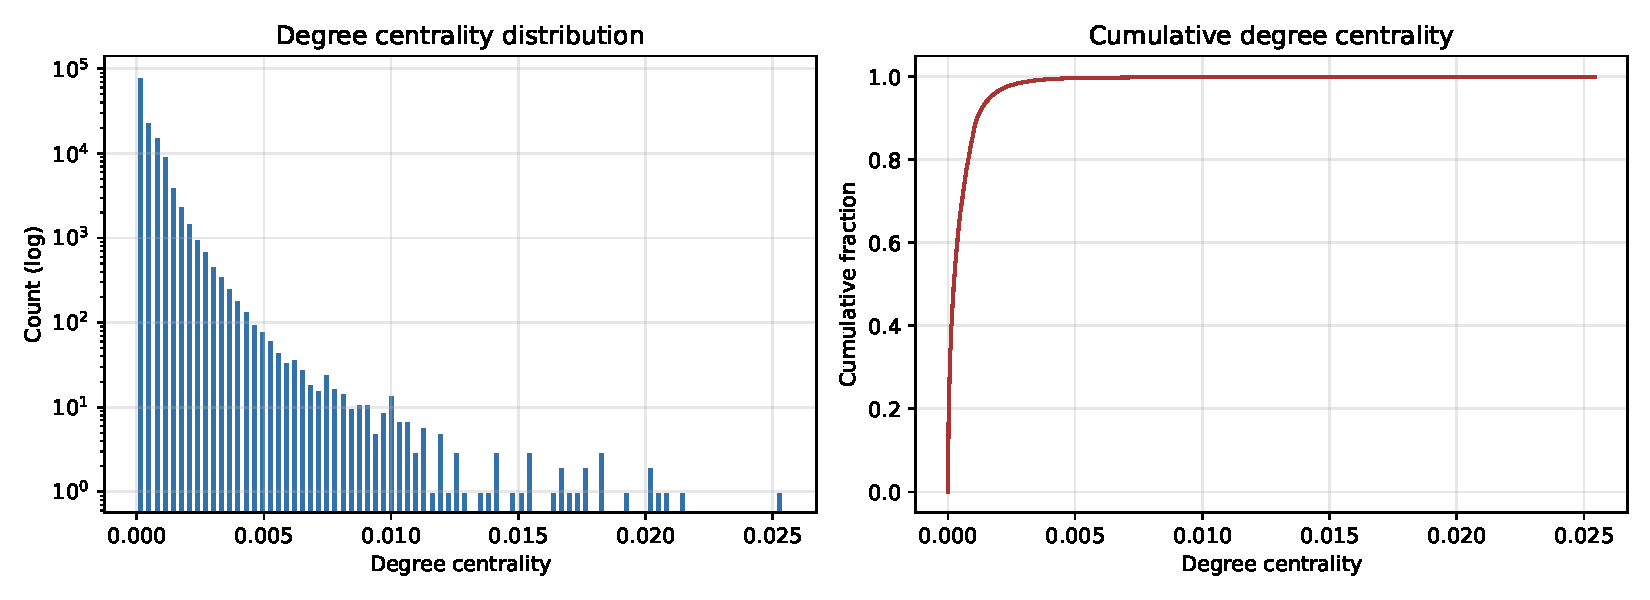
\includegraphics[width=\linewidth]{task4_degree_distributions.pdf}
    \column{0.5\linewidth}
    \centering
    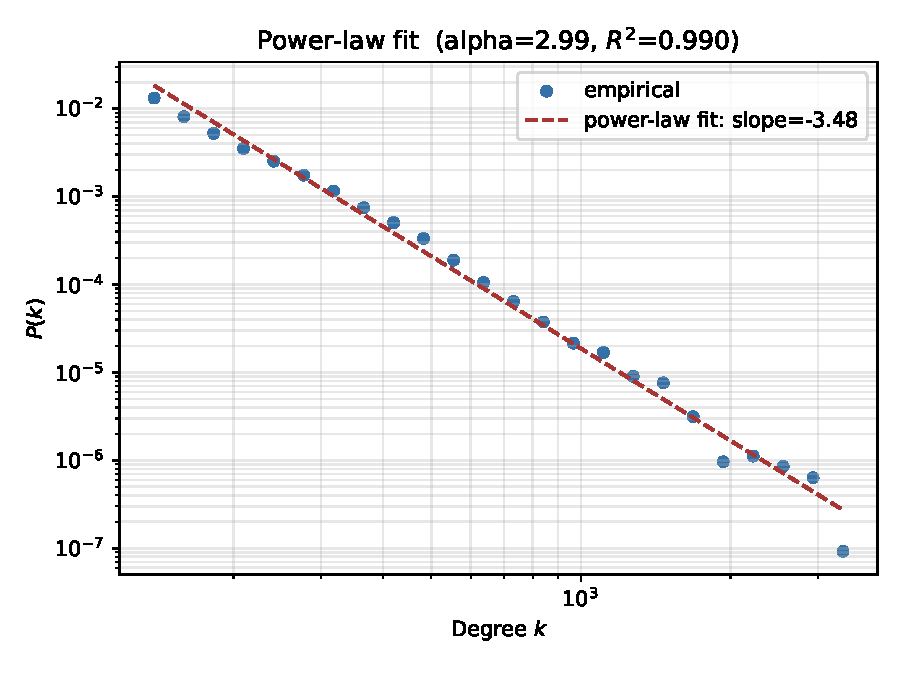
\includegraphics[width=\linewidth]{task5_powerlaw.pdf}
  \end{columns}
  \vfill
  \footnotesize
  \begin{itemize}
    \item \texttt{powerlaw.Fit} (Clauset--Shalizi--Newman MLE):
          \(\alpha = \mathbf{2.99}\), \(x_{\min}=116\)
    \item log-binned tail regression: slope \(=-3.48\),
          \(\boldsymbol{R^{2}=0.99}\)
    \item \alert{but} \texttt{distribution\_compare} prefers
          \emph{lognormal} over power-law\\
          (\(R = -10.6\), \(p < 10^{-25}\)) -- consistent with
          Broido \& Clauset 2019.
  \end{itemize}
\end{frame}

% ---------------------------------------------------------------- 8. Time decomposition
\begin{frame}{Temporal decomposition (10 increments)}
  \begin{columns}[T,onlytextwidth]
    \column{0.46\linewidth}
    \centering
    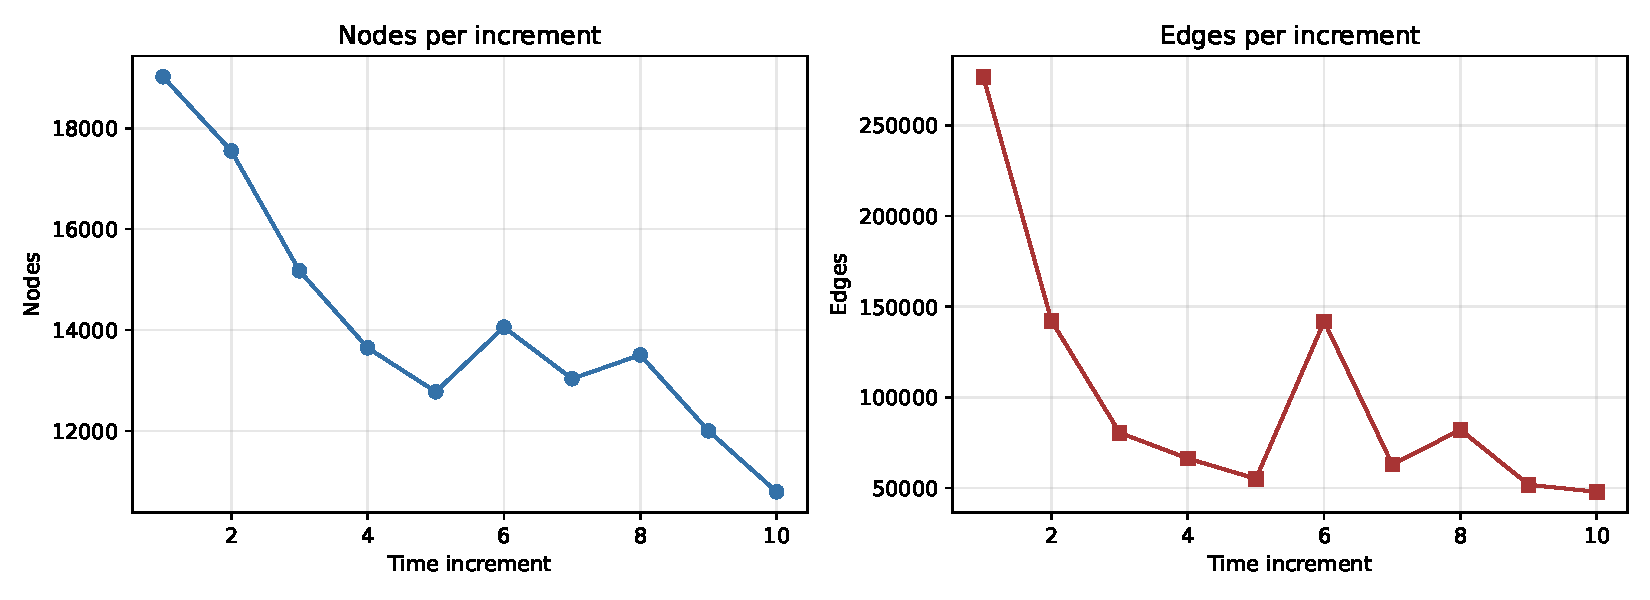
\includegraphics[width=\linewidth]{task6_subgraph_evolution.pdf}
    \column{0.54\linewidth}
    \footnotesize
    \begin{tabular}{rrrrr}
      \toprule
      \(t\) & \(|V|\) & \(|E|\) & avg path & diam \\
      \midrule
      1 & 19\,022 & 276\,860 & 3.71 & 9 \\
      2 & 17\,552 & 142\,257 & 4.56 & 12 \\
      3 & 15\,175 &  80\,482 & 4.92 & 11 \\
      4 & 13\,647 &  66\,330 & 5.08 & 14 \\
      5 & 12\,776 &  55\,102 & 5.38 & 13 \\
      6 & \alert{14\,057} & \alert{141\,915} & 5.16 & 13 \\
      7 & 13\,034 &  62\,926 & 5.82 & 12 \\
      8 & 13\,506 &  82\,158 & 5.88 & 14 \\
      9 & 12\,001 &  51\,806 & 5.99 & 14 \\
      10 & 10\,792 &  47\,913 & 6.00 & 16 \\
      \bottomrule
    \end{tabular}
  \end{columns}
  \vfill
  \footnotesize
  Network \emph{shrinks and elongates} over the period;
  \alert{rebound at \(t\!=\!6\)} aligns with the
  U.S.\ impeachment public hearings (mid-November).
\end{frame}

% ---------------------------------------------------------------- 9. Subgraph drawings
\begin{frame}{Subgraph LCC drawings}
  \centering
  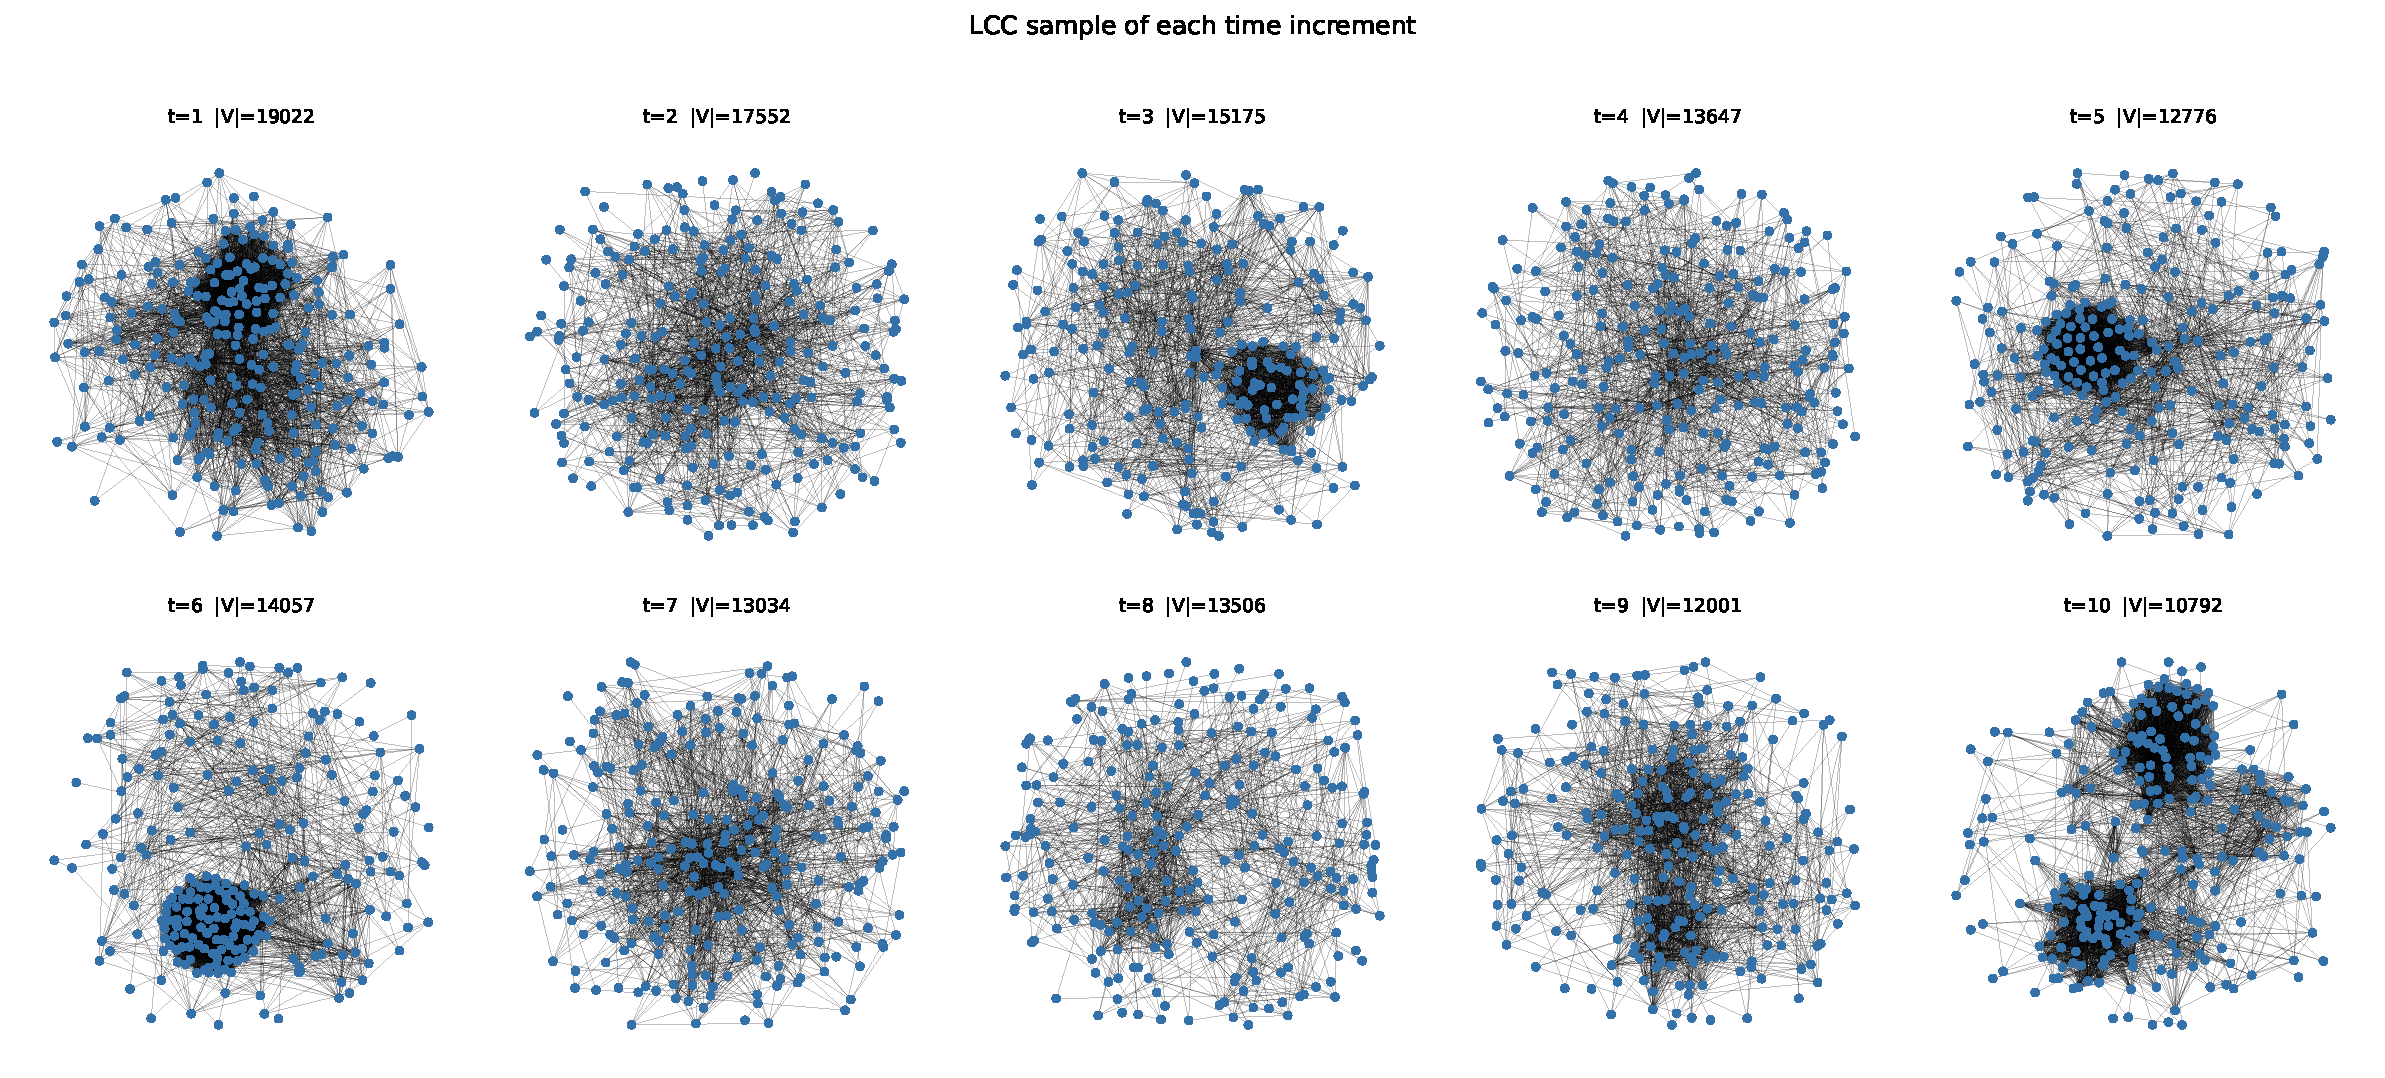
\includegraphics[width=0.95\linewidth]{task6_subgraph_drawings.pdf}
  \vspace{2pt}\\
  \footnotesize
  Each panel: largest CC of one increment, BFS-down-sampled to
  250 nodes for legibility.  Topology drifts from
  hub-and-spoke towards chain-like as cohorts shrink.
\end{frame}

% ---------------------------------------------------------------- 10. Triangles
\begin{frame}{Triangle evolution}
  \begin{columns}[c,onlytextwidth]
    \column{0.6\linewidth}
    \centering
    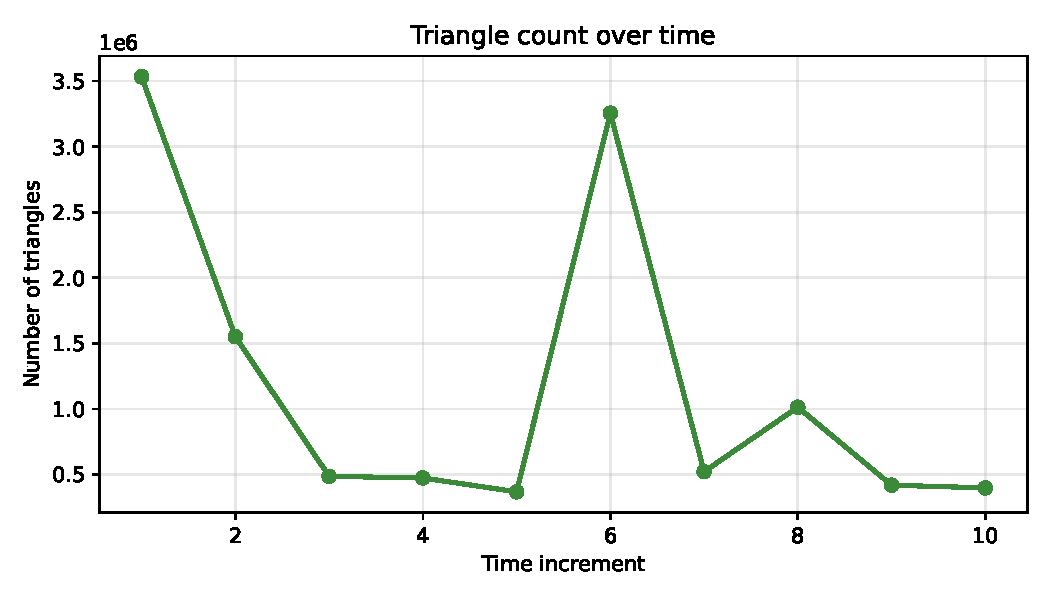
\includegraphics[width=\linewidth]{task7_triangles.pdf}
    \column{0.4\linewidth}
    \footnotesize
    \begin{tabular}{rr}
      \toprule
      \(t\) & Triangles \\
      \midrule
      1 & \alert{3\,533\,557} \\
      2 & 1\,551\,246 \\
      3 &    486\,032 \\
      4 &    473\,306 \\
      5 &    367\,686 \\
      6 & \alert{3\,255\,905} \\
      7 &    521\,393 \\
      8 & 1\,013\,158 \\
      9 &    418\,406 \\
      10 &   397\,780 \\
      \bottomrule
    \end{tabular}
  \end{columns}
  \vfill
  \footnotesize
  October cohorts are densely tri-connected; the
  \alert{\(t\!=\!6\) rebound} mirrors the size rebound and
  reflects the impeachment-news clustering.
\end{frame}

% ---------------------------------------------------------------- 11. Sentiment
\begin{frame}{Sentiment evolution}
  \begin{columns}[T,onlytextwidth]
    \column{0.55\linewidth}
    \centering
    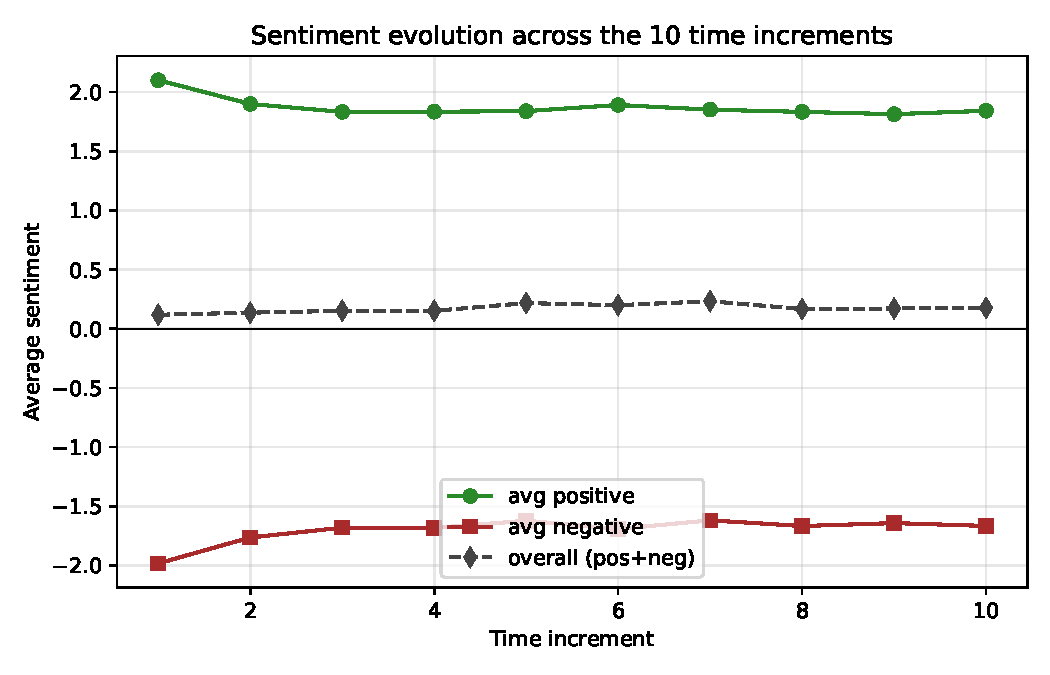
\includegraphics[width=\linewidth]{task8_sentiment.pdf}
    \column{0.45\linewidth}
    \footnotesize
    \textbf{Per-increment aggregation:}
    \[
      s = s^{+} + s^{-},\;
      \overline{s_i} =
      \tfrac{1}{|V_i|}\!\sum_{u\in V_i}\!\sum_{\tau \in T_i(u)} s(\tau)
    \]
    \begin{itemize}\itemsep2pt
      \item per-node \(\overline{s^{+}}\!\approx\!+1.9\),
            \(\overline{s^{-}}\!\approx\!-1.7\)
      \item overall sentiment mildly positive\\
            (\(\sim\!+0.12\) to \(+0.23\))
      \item \(\sum |s^{-}_t|\) \emph{volume} drops from
            \(\sim\!104\)k (\(t\!=\!1\)) to \(\sim\!18\)k
            (\(t\!=\!10\)) -- driven by the shrinking active
            user base.
    \end{itemize}
  \end{columns}
\end{frame}

% ---------------------------------------------------------------- 12. SIS
\begin{frame}{SIS calibration}
  \begin{columns}[T,onlytextwidth]
    \column{0.55\linewidth}
    \centering
    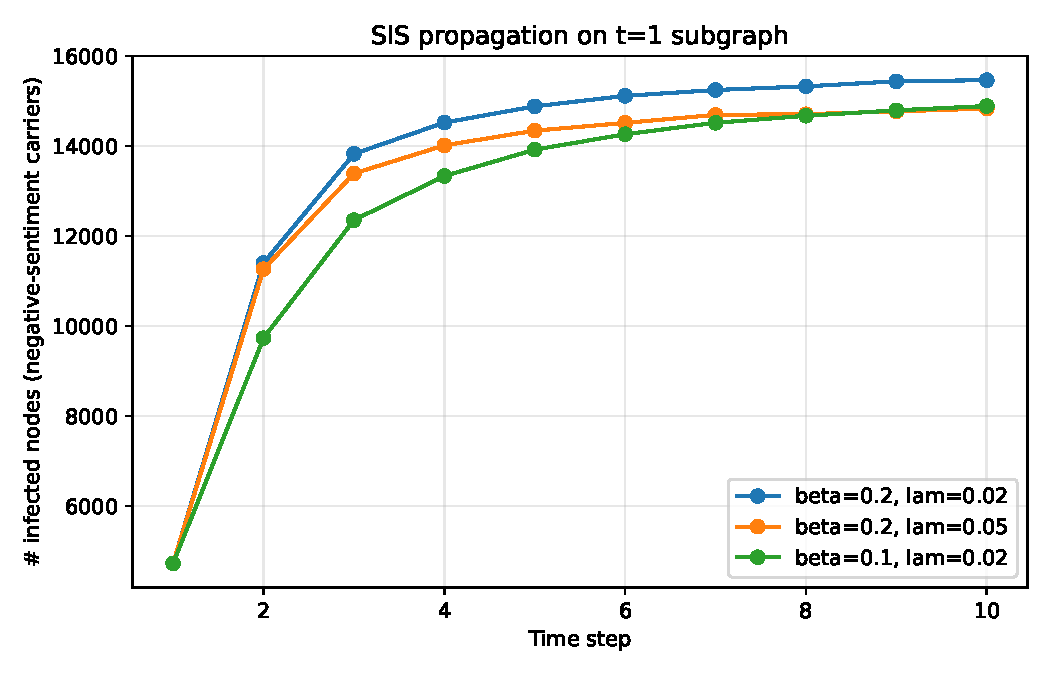
\includegraphics[width=\linewidth]{task9_sis_topfits.pdf}
    \column{0.45\linewidth}
    \scriptsize
    \begin{tabular}{rrrr}
      \toprule
      \(\beta\) & \(\lambda\) & Final & Cumul. \\
      \midrule
      0.20 & 0.02 & 15\,443 & \alert{135\,754} \\
      0.20 & 0.05 & 14\,852 & 131\,537 \\
      0.10 & 0.02 & 14\,821 & 126\,727 \\
      0.20 & 0.10 & 13\,915 & 124\,692 \\
      0.10 & 0.05 & 14\,146 & 122\,560 \\
      \bottomrule
    \end{tabular}
    \vspace{4pt}
    \footnotesize
    \begin{itemize}
      \item Host: LCC of \(t\!=\!1\) subgraph
            (16\,036 nodes, 274 k edges)
      \item target \(\sum |s^{-}_t| = 242\,901\)
      \item best fit reaches \alert{\(\sim\)56\,\%}
      \item structural ceiling: cum.\ infections
            \(\le 10|V| \approx 1.6\!\times\!10^{5}\)
    \end{itemize}
  \end{columns}
\end{frame}

% ---------------------------------------------------------------- 13. Limitations
\begin{frame}{Honest limitations \& deviations}
  \begin{block}{Three deliberate departures from the literal spec}
    \begin{enumerate}\itemsep2pt
      \item[1.] \textbf{150-fanout cap} -- otherwise the
            BFS-bound metrics take hours, not minutes
      \item[2.] \textbf{Sampled} avg path / diameter
            (\(|S|=200/60/20\)) instead of exact NetworkX call
      \item[3.] \textbf{matplotlib drawings} replace
            ``Delphi visualisation'' (likely typo for Gephi)
    \end{enumerate}
  \end{block}
  \vfill
  \begin{itemize}\itemsep2pt
    \item \textbf{Hashtag-projection bias:} co-occurrence
          \(\neq\) information transfer.
    \item \textbf{Power-law caveat:} lognormal favoured
          formally; we report both honestly.
    \item \textbf{Sentiment \(\neq\) pathogen:} news shocks
          are exogenous, SIS only matches volume, not cause.
    \item \textbf{Pre-pandemic window:} Oct--Nov 2019 is a
          baseline, not a pandemic snapshot.
  \end{itemize}
\end{frame}

% ---------------------------------------------------------------- 14. Conclusion
\begin{frame}{Conclusions \& future work}
  \begin{block}{What we learned}
    \begin{itemize}\itemsep2pt
      \item \(G\) is heavy-tailed, small-world, dominated by a
            \(\sim\!94\%\) giant component.
      \item Power-law \(\alpha\!\approx\!3\), \(R^{2}\!=\!0.99\),
            \alert{but} lognormal preferred.
      \item Cohorts \emph{shrink and elongate} from October to
            late November, with a clear mid-November
            rebound.
      \item Triangle counts mirror the size rebound; sentiment
            stays mildly positive.
      \item SIS contagion captures \(\sim\!56\%\) of cumulative
            negative volume \(\rightarrow\) shape ok, cause
            unrecoverable.
    \end{itemize}
  \end{block}
  \begin{block}{Next steps}
    \begin{itemize}\itemsep2pt
      \item temporal bipartite mention/retweet graph
      \item joint positive/negative epidemics
      \item rerun on the post-March-2020 window for a
            pre-vs-pandemic diff
    \end{itemize}
  \end{block}
\end{frame}

% ---------------------------------------------------------------- 15. Q&A
\begin{frame}[c]
  \begin{center}
    {\Huge \color{accent}\textbf{Questions?}}\\[14pt]
    \href{https://github.com/MatusMandzak/sna-project}%
      {\texttt{github.com/MatusMandzak/sna-project}}\\[6pt]
    \footnotesize \texttt{matus.mandzak@student.oulu.fi}
  \end{center}
\end{frame}

\end{document}
